\chapter{健康习惯}\label{ch:g1:healthy-habits}

为什么大家总是说“洗手”“刷牙”“该睡觉了”？
这可不是为了扫兴。你的身体是你要用得最久的“\omterm{def:g1:living-or-not:living}{生物}”——
要用一辈子——每天坚持几个小习惯，
就能让它保持强健。下面说说这些习惯是什么，
以及它们为什么有用。

\section{保持清洁}

\begin{definition}[病菌]\label{def:g1:healthy-habits:germs}
\emph{病菌}\index{病菌}是一些小到肉眼看不见的\omterm{def:g1:living-or-not:living}{生物}，
它们无处不在——手上、门把手上、泥土里都有。大多数病菌无害，
但有些病菌一旦进入人体，就会让人生病。
因为病菌看不见，看起来干净的手，
也可能带着它们。
\end{definition}

\begin{definition}[卫生]\label{def:g1:healthy-habits:hygiene}
\emph{卫生}\index{卫生}指的是让身体保持清洁的习惯，
也就是让\omterm{def:g1:healthy-habits:germs}{病菌}远离身体，包括洗手、洗澡、刷牙，
以及保持食物清洁。
\end{definition}

\begin{method}[正确洗手]\label{met:g1:healthy-habits:hands}
\begin{enumerate}
  \item 把手弄湿，取适量肥皂；
  \item 搓遍双手——手心、手背、指缝之间、
        大拇指周围——慢慢数到 $20$，
        或者唱一首短歌；
  \item 在流动的水下冲洗干净；
  \item 用干净的毛巾擦干。
\end{enumerate}
饭前、上厕所后，以及在外面玩耍后，
或摸过\omterm{def:g1:animals-around-us:animal}{动物}之后，都要洗手。
\end{method}

\begin{omfigure}
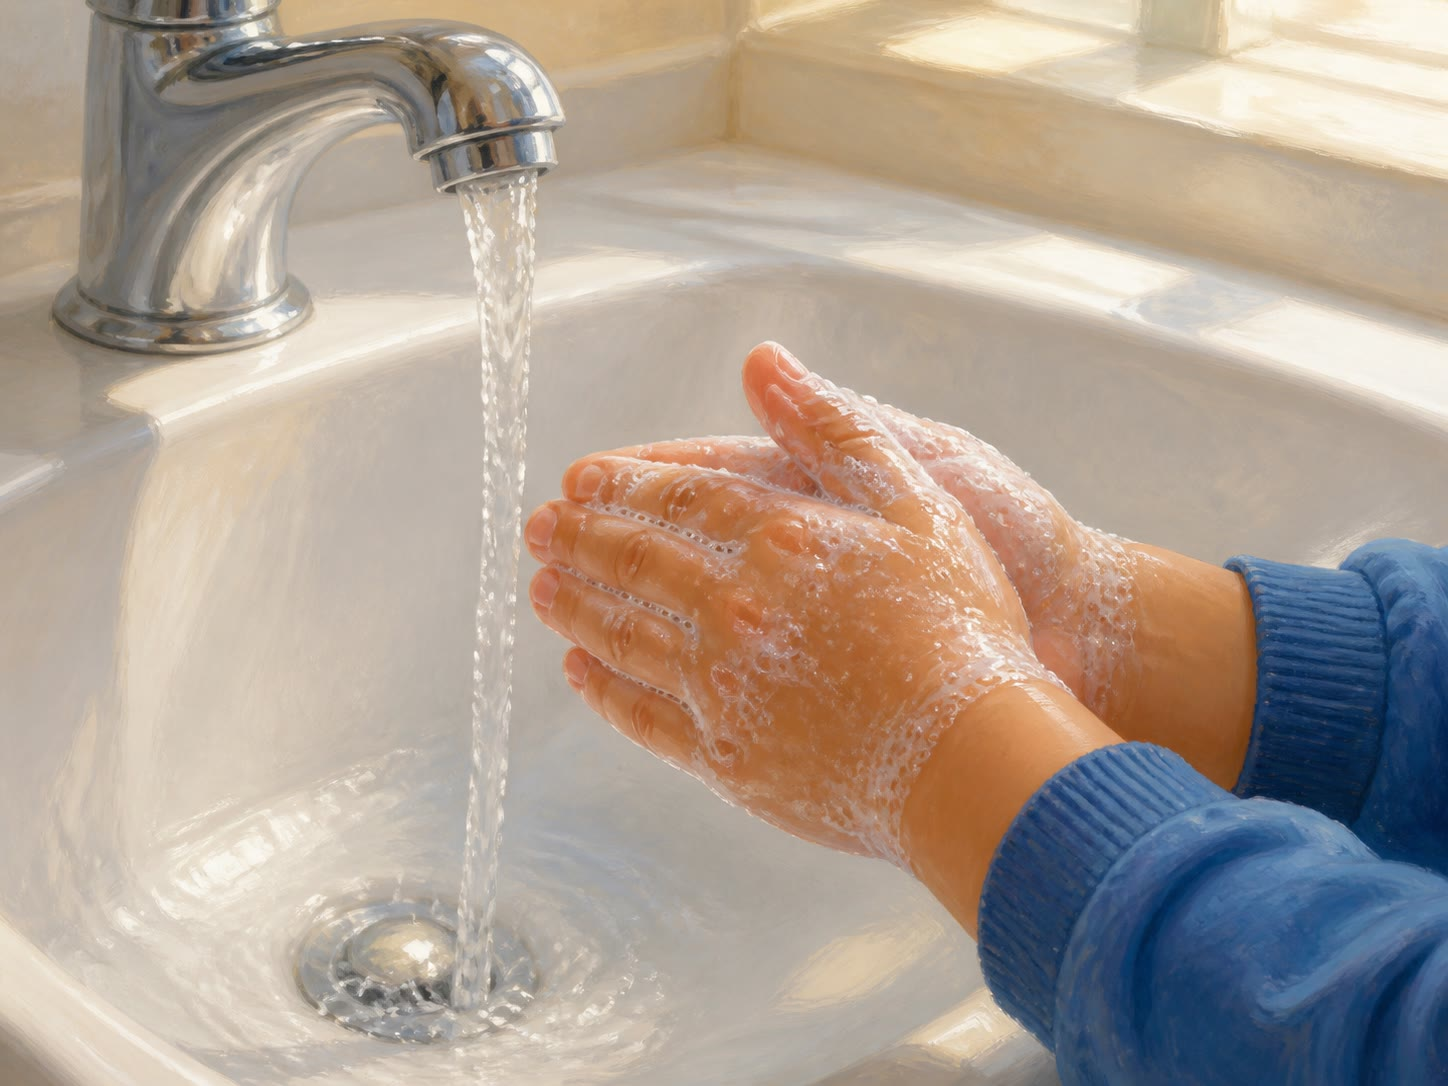
\includegraphics[width=0.58\linewidth]{images/book1/ai/g1-habits-handwashing.jpg}

{\small 肥皂、搓洗、流水：\omterm{def:g1:healthy-habits:germs}{病菌}最讨厌的“歌”，
只要慢慢数到二十。}
\end{omfigure}

\begin{example}[闪粉实验]\label{ex:g1:healthy-habits:glitter}
在手心上抹一小撮闪粉，然后和朋友握手、开门、拿铅笔，
闪粉就到处都是。\omterm{def:g1:healthy-habits:germs}{病菌}也是这样传播的，
只是我们看不见。现在用肥皂洗手，
数到 $20$——闪粉没了，\omterm{def:g1:healthy-habits:germs}{病菌}也就没了。
\end{example}

\section{保护牙齿}

\begin{proposition}[为什么要刷牙]\label{prop:g1:healthy-habits:teeth}
吃完东西后，牙齿上会留下食物碎屑。口腔里的\omterm{def:g1:healthy-habits:germs}{病菌}
以这些残渣为食，尤其是甜的食物，慢慢在牙齿上蛀出洞来，
而且会疼。刷牙可以在\omterm{def:g1:healthy-habits:germs}{病菌}大快朵颐之前，
把这些残渣清除掉。
\end{proposition}
\admitted

\begin{method}[刷牙]\label{met:g1:healthy-habits:brush}
\begin{enumerate}
  \item 每天早饭后和睡觉前都要刷牙；
  \item 每颗牙的每一面都要刷到：前面、后面，
        以及用来咀嚼的顶面；
  \item 慢慢刷，大约和唱一首歌的时间一样长；
  \item 刷毛岔开时，就换一把新牙刷。
\end{enumerate}
\end{method}

\begin{remark}[乳牙也很重要]\label{rem:g1:healthy-habits:babyteeth}
“这些牙反正会掉，为什么还要刷？”因为它们还要替你咀嚼好多年，
因为牙上的蛀洞一样会疼，还因为恒牙已经在下面等着，
而且恒牙
值得在干净、健康的口腔里长出来。
\end{remark}

\section{饮食、运动与睡眠}

\begin{proposition}[每天的三项需要]\label{prop:g1:healthy-habits:needs}
正在成长的身体每天都需要：
\begin{enumerate}
  \item \emph{多样的食物}\index{多样的食物}——各种食物都吃一点：蔬菜和水果、面包和谷物，
        牛奶和奶酪、肉、鱼或蛋，
        还要喝水；
        甜食只偶尔吃一点；
  \item \emph{运动}\index{运动}——跑步、攀爬、骑车、在户外玩耍：
        运动可以让肌肉、骨骼
        和心脏变得更强壮；
  \item \emph{睡眠}\index{睡眠}——夜里身体休息，
        自我修复并生长；儿童需要的夜间\omterm{prop:g1:healthy-habits:needs}{睡眠}，
        比成年人长得多。
\end{enumerate}
\end{proposition}
\admitted

\begin{omfigure}
\begin{tikzpicture}
  \draw[thick, omMeth, fill=omMeth!7, rounded corners=6pt]
    (0,0) rectangle (3.6,2.3);
  \draw[thick, omProp, fill=omProp!7, rounded corners=6pt]
    (4.0,0) rectangle (7.6,2.3);
  \draw[thick, omDef, fill=omDef!7, rounded corners=6pt]
    (8.0,0) rectangle (11.6,2.3);
  \node[font=\small\bfseries, omMeth] at (1.8,1.95) {多样饮食};
  \node[font=\small\bfseries, omProp] at (5.8,1.95) {运动};
  \node[font=\small\bfseries, omDef] at (9.8,1.95) {睡眠};
  \node[font=\small, align=center, text width=3.3cm] at (1.8,0.9)
    {每样都吃一点，\\ 多喝水};
  \node[font=\small, align=center, text width=3.3cm] at (5.8,0.9)
    {户外玩耍，\\ 跑步、攀爬，\\ 每天都做};
  \node[font=\small, align=center, text width=3.3cm] at (9.8,0.9)
    {夜里好好睡，\\ 身体修复 \\ 并生长};
\end{tikzpicture}

{\small 生长中身体的三项日常需求。三者
互不能替代。}
\end{omfigure}

\begin{example}[身体的美好一天]\label{ex:g1:healthy-habits:day}
早餐吃水果，午饭前洗手，下午在公园里跑步，
晚饭后刷牙，早早关灯，听一个故事。
没有什么特别之处——而这正是要点：
健康正是由像这样普通的日子构成的。
\end{example}

\begin{remark}[疲劳也是一种信号]\label{rem:g1:healthy-habits:tired}
打哈欠、眼睛发酸、无缘无故闹脾气，这都是身体在说
“我需要睡觉”。听从它的提醒，也是一种健康的习惯。
睡足了的早晨，大脑学得更好，玩得更好，
也更容易笑起来。
\end{remark}

\section{练习}

\begin{exercise}[$\star$]\label{exo:g1:healthy-habits:1}
什么是\omterm{def:g1:healthy-habits:germs}{病菌}？为什么看起来干净的手仍然需要洗？
\end{exercise}

\begin{exercise}[$\star$]\label{exo:g1:healthy-habits:2}
说出一天中必须洗手的三个时刻。
\end{exercise}

\begin{exercise}[$\star$]\label{exo:g1:healthy-habits:3}
在\cref{met:g1:healthy-habits:hands}中，
用肥皂搓手应持续多长时间？说出两个容易忘记的部位。
\end{exercise}

\begin{exercise}[$\star$]\label{exo:g1:healthy-habits:4}
牙齿不刷，为什么会长出空洞？
请结合\omterm{def:g1:healthy-habits:germs}{病菌}和食物残渣，讲一讲这个过程。
\end{exercise}

\begin{exercise}[$\star$]\label{exo:g1:healthy-habits:5}
什么时候应该刷牙？每次应刷多长时间？
\end{exercise}

\begin{exercise}[$\star$]\label{exo:g1:healthy-habits:6}
说出\cref{prop:g1:healthy-habits:needs}中的三项日常需求，
并从你自己的一天中各举一个例子。
\end{exercise}

\begin{exercise}[$\star$]\label{exo:g1:healthy-habits:7}
\omterm{prop:g1:healthy-habits:needs}{睡眠}时身体会做些什么？
小孩还是大人，谁需要更长的夜晚？
\end{exercise}

\begin{exercise}[$\star$]\label{exo:g1:healthy-habits:8}
说出身体在请求\omterm{prop:g1:healthy-habits:needs}{睡眠}的两个信号。
\end{exercise}

\begin{exercise}[$\star\star$]\label{exo:g1:healthy-habits:9}
萨姆说：“反正乳牙迟早会掉，
所以刷它们没有用。”请用
\cref{rem:g1:healthy-habits:babyteeth}回答他——至少给出两条理由。
\end{exercise}

\begin{exercise}[$\star\star$]\label{exo:g1:healthy-habits:10}
在\cref{ex:g1:healthy-habits:glitter}的闪粉实验中，
闪粉代表什么？这个实验说明了关于
握手——以及肥皂的哪些道理？
\end{exercise}
